{\bf ADD REFERENCES}

The technology most widely used today in digital fractional order
circuitry is the continued fraction expansion (CFE) approximation to
$s^\alpha$. Its benefits are that it was a flat phase response over
approximately two and a half decades in phase for a 9th order
expansion (10 registers of input signal memory). It would be desirable
to find an algorithm with an even broader flat phase frequency
bandwidth and with a comparably small amount of memory required. We
take the Grunwald algorithm as a starting point. As the signal history
retained in the Grunwald sum grows longer, the bandwidth of flat phase
response grows broader; however, the memory required also increases
with input signal history length. To reduce this memory requirement
and retain a long signal history, we propose partitioning the input
signal history into bins that are longer further into the past. The
value of the binned input signal is represented by the average value
of the input signal within that bin. The presence of short bins at
recent times maintains sensitivity to high frequencies, while the
inclusion of long bins at past times adds sensitivity to low
frequencies that would not usually be present in a Grunwald sum with
the same number of terms. (See Figure~\ref{fig:freqScaling}).

\begin{figure}
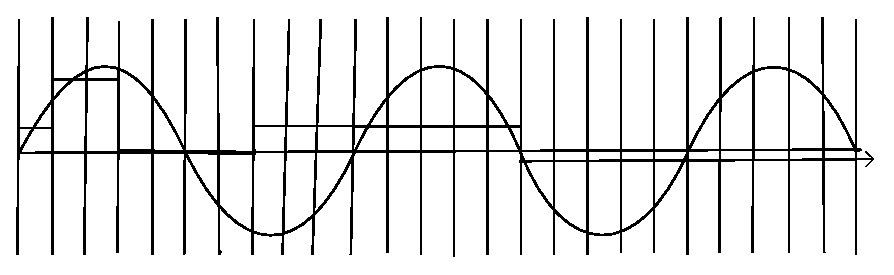
\includegraphics[width=3in]{sensitivityIsFreqDependent.eps}
\label{fig:freqScaling}
\caption{Let each division represent a single time step and each bar represent a bin, scaled such that the duration of a bin increases further back in time (toward the right). The value of the bin is the average of the input signal, the sine wave, at each point in time within that bin. There exists some oldest bin that responds sensitively to the input signal (in this figure, the second bin). For lower frequencies, that oldest bin moves to older times. This illustrates the sensitivity of short bins at recent times to high frequencies and long bins in the distant past to low frequencies.}
\end{figure}


\subsection{Modified Grunwald}

The Grunwald form of the fractional integral can be written

\begin{equation}
_0D^\alpha_tf(t) = \displaystyle \lim_{N\to\infty} \left(\frac{t}{N_t}\right)^{-\alpha}
\displaystyle\sum\limits_{j=0}^{N_t-1} w_{j}x_j
\label{simpleGrunwald}
\end{equation}
where $f(t)$ is the input signal at time $t$, the $j$th value of the
input signal history is $x_j=f\left(t-\frac{j\Delta t}{N_t}\right)$, and the
$j$th Grunwald weight is

\begin{equation}
w_{j} = \frac{\Gamma(j-\alpha)}{\Gamma(j+1)\Gamma(-\alpha)}.
\label{wj}
\end{equation}
To include more distant history at low computational cost, we modify
the Grunwald sum of Equation~\ref{simpleGrunwald} by partitioning its
history into $N_b$ bins. In each bin $k$, the input signal history
$x_j$ is represented by its average value over that bin, $X_k$.

Since we make the assumption that each value is well represented by
its average within a bin, we can define a value for the "bin
coefficient" by summing the Grunwald coefficients within that bin.

\begin{equation}
W_k = \displaystyle\sum\limits_{j=p_{k-1}+1}^{p_k} w_j
\label{eqn:sumWk}
\end{equation}

\noindent where $w_j$ is summed from the lowest index of the input data history within bin $k$ to the highest index $p_k$ within that bin. There is an additional factor that goes into $\bar{W}$ that will be discussed in Section~\ref{sec:shifting}. 

With these definitions, the modified Grunwald differ-integral can be written

\begin{equation}
_0D^\alpha_t f(t) = \displaystyle(\Delta t)^{-\alpha}\sum\limits_{k=0}^{N_b}\bar{W}_kX_k
\label{avgSimpleGrunwald}
\end{equation}
where $\Delta t$ is the interval between time samples.



\subsection{Updating the average history}
\label{sec:shifting}

When a new input data element is read, the history is updated. The new data element is shifted into the first bin through a weighted average. Since data elements represent time steps, they should be incompressible-- when one element is shifted into a bin, another virtual element should be shifted out of that bin if the bin is full. It shifts into the next bin, and pushes a virtual element out of that one, until a bin which is partially full or empty is reached. To update the average data stored in the bins, we take the weighted average obtained by adding one virtual element from the $(k-1)$th bin to the $b_k$ elements in the $k$th bin. This process is illustrated in Figure~\ref{fig:binShifting}.

\begin{figure}
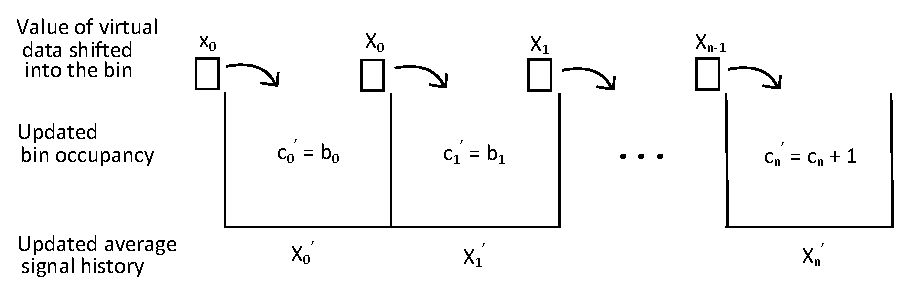
\includegraphics[width=4in]{binShifting.eps}
\label{fig:binShifting}
\caption{When the input data $x_0$ is read, virtual data elements with bin average values $X_k$ are shifted from the $k$th to the $(k+1)$th bin. The first $n-1$ bins are at capacity, but the $n$th bin gains one data point. The bin averages are updated to value $X_k^\prime$ through a weighted average.}
\end{figure}

During start-up, it will be necessary to consider bins that have some
set size $b_k$, but are not filled to that capacity. In that case, it
is the current occupation number $c_k$ of each bin that enters the
calculation. If the $k$th bin initially contains $c_k$ elements,
updating the history either leaves $c_k$ ($c_k\prime=c_k=b_k$) or
increments the number of elements in the bin such that $c_k\prime =
c_k + 1$ if the bin is not yet at capacity. Either way, the updated
average of the value of the $k$th bin, $X_k\prime$, is given by

\begin{equation}
X_k^\prime = \frac{c_k^\prime-1}{c_k^\prime}X_k + \frac{1}{c_k^\prime}X_{k-1}.
\label{eqn:updating}
\end{equation}
where $X_{-1}$ is taken to be $x_0$, the input data that has just been
read. 

During start-up, these partially full bins may also factor into
the Grunwald weights. To handle bins that are partially full, we
weight the binned Grunwald weights by the ratio of the bin occupation
number $c_k$ to its capacity $b_k$,

\begin{equation}
\bar{W}_k= \frac{c_k W_k}{b_k}.
\label{eqn:Wbar}
\end{equation} 









